\section{Technical Background}
\label{sec:state:technical}
This chapter will give us an overview of important mechanisms used by modern
CPUs. While there are other widely used architectures, such as ARM on
mobile devices, we will explore these features in the example of the x86\_64
architecture. \\

We decided to do so because our proof of concept implementation will target
the x86\_64 architecture. Moreover, behavior and implementations of similar
concepts can differ between \gls{isa} (\acrshort{a_isa}) and even
implementations of the same \acrshort{a_isa} on the microarchitectural plane.
We will, therefore, note differences in implementations of x86\_64 whenever
appropriate. Until then, we will stick to the general behavior described in
the AMD64 specification so that the Intel 64-bit extensions are largely
compatible.

\subsection{Operation Modes}
\label{sec:state:technical:modes}
The x86 architecture is rooted in the Intel 8086, designed in 1978. As
a 16-bit microprocessor design, the Intel 8086 physically can only address 64
KiB of memory. To overcome this limitation, Intel introduced a
segmentation-based addressing mode that, together with the 20-bit address bus,
allowed the CPU to address slightly more than 1 MiB of main memory. Intel 8086
missed features such as memory protection, code privileges, and multitasking.
These features were important to allow advanced operating systems. These
features extended the instruction set and microarchitecture
implemented by the Intel 80286. The Intel 80286 could address, for example,
16 MiB of physical memory through 24 address bus bits and could address 1 GiB of
virtual memory. Moreover, segment registers now contain an index in a
data structure called \gls{gdt}, short \acrshort{a_gdt}.
The \acrshort{a_gdt} contains descriptors that store information on segments,
such as base address and access rights. The Intel 80286 implements access rights
as so-called rings, and the lower the numerical access level, the higher the
privileges of the executing software are. The introduction of the
\acrshort{a_gdt} allowed virtual memory implementation with memory protection.
A new \gls{mmu}, short \acrshort{a_mmu}, added for the first time on chip in
the 80286 allowed fast virtual to physical address translation. \\

When using the features newly added to the 80286
the processor was incompatible with the original Intel 8086. Because the result
would have been that all software already existing for the Intel 8086 would have
been to at least be recompiled to run on the Intel 80286, Intel designed the new
features as an extension to the older 8086. Deactivating these new features
allowed the Intel 80286 to run programs written for the 8086. For this, Intel
introduced two operation modes in the 80286. The operation mode offering
compatibility was called \textbf{\gls{rmode}} because the address
calculation in the 8086 always yielded real physical addresses. Because the new
80286 offered memory protection, the mode was called \textbf{\gls{pmode}}. To
maintain compatibility with the Intel 8086, the 80286 first boots in
\gls{rmode}, as all successors of the 80286 do. On startup, the code for
entering other operation modes must, therefore, reside in the first MiB of
memory. \\

The successor of the Intel 80286, the Intel 80386 extended the architecture to
32-bit and introduced paging to the architecture, allowing paged virtual memory
(cf. \ref{sec:state:technical:paging}). The registers of the 80386 were also
extended to 32-bit. To differentiate between the registers and their extensions,
they are prefixed with ''E''. For example, the instruction pointer register,
formerly identified by IP, becomes EIP with. The Intel 80386 also added the
\textbf{\gls{smm}} or short \acrshort{a_smm}. The \acrshort{a_smm} is intended
for firmware to execute special tasks such as energy management or other tasks
executed by the firmware. The \acrshort{a_smm} code resides in a specially
protected area of the main memory, referred to as \gls{smram}. \acrshort{a_smm}
executes with the highest privileges in x86, which is ring -2. With these
changes, the Intel 80386 formed the base for the architecture today known as x86
or IA-32.\\

Successors of the 80386 added support for optional floating point units and
\acrshort{a_simd} extensions to the architecture but left the fundamental
\acrshort{a_isa} unchanged. It was not until the year 2000 that AMD released
its extensions of the x86 architecture to 64 bit that introduced a new processor
operation mode called \textbf{\gls{lmode}} and two sub modes called
\textbf{Compatibility Mode} and \textbf{64-Bit mode}. This extension by AMD to
the x86 \acrshort{a_isa} was first called AMD64 and later largely adopted by
Intel as Intel 64. Today it is also known by the name x86\_64.
Compatibility mode allows the execution of legacy 32-bit and 16-bit code.
64-bit mode extends the \acrshort{a_isa} by 64-bit operands and addresses, and
extends all general purpose registers to 64-bit. Moreover, the 64-bit mode
adds eight additional general-purpose registers and allows instruction pointer
relative addressing. x86 allowed the latter only in control transfer
instructions. AMD64 implements floating-point arithmetic through the mandatory
SSE2 \acrshort{a_simd} extension that was introduced to x86 in 2000 with the Intel
Pentium 4 processor. The number of SSE2 registers is doubled compared to the
number in the original x86 extension. Moreover, to allow differentiating between
x86 and AMD64 registers, AMD added the REX prefix to the specification. As a
result, general purpose registers are prefixed with the letter ''R''. For
example, the instruction pointer registers of x86 (IP) becomes RIP. The number
of page table levels to translate virtual to physical addresses was increased
from two to at least four.\\

Unless otherwise stated, all references we make to \gls{lmode} in
the remaining parts of this thesis mean the combination of both sub-modes and
therefore the whole extension implemented by AMD64.

\subsection{Interrupts and Exceptions}
\label{sec:state:technical:interrupts}
Interrupts and Exceptions are used to call system-specific functions and respond
to special conditions in the CPU or system. Exceptions occur while executing
software and result from program or CPU internal errors. Interrupts, on the
other hand, are either the result of software interrupt instructions or the
interaction of the CPU with other system components, such as keyboard input.
Exceptions can be divided into three types:
\begin{enumerate}
    \item Faults: Result of an error with the instruction to execute
    \item Traps: Result of breakpoint and software interrupt instructions
    \item Aborts
\end{enumerate}
Interrupts, on the other hand, can be divided into two classes:
\begin{enumerate}
    \item Maskable Interrupts: Can be masked. Masking an interrupt means that
          software can temporarily disable them. The interrupt controller
          holds them back until interrupts are enabled again.
    \item \Gls{nmi}~(\acrshort{a_nmi}): Software cannot
          turn off \acrshort{a_nmi}s. The interrupt controller delivers~
          \acrshort{a_nmi}s to the CPU unless it currently serves another~
          \acrshort{a_nmi}. When the CPU executes the IRET instruction in the
          interrupt handler, the interrupt controller can deliver the next~
          \acrshort{a_nmi}.
\end{enumerate}
The CPU serves exceptions and interrupts by calling the respective interrupt or
exception handler routine. System software can install an interrupt handler by
writing its address into the \gls{idt}, short \acrshort{a_idt}. The
\acrshort{a_idt} is a data structure containing pointers to interrupt handling
routines. The specification assigns a so-called vector to each interrupt or
exception. With the help of this vector, the CPU determines what handler to call
by using the interrupt vector as an index in the \acrshort{a_idt}. It finds the
\acrshort{a_idt} by reading the value of the interrupt descriptor table register
(IDTR). System software is expected to create the \acrshort{a_idt} and install
handlers for at least the predefined vectors. Then, the address of the
\acrshort{a_idt} will be provided by writing to the IDTR before interrupts can
be activated. \\

Over time, interrupt controllers were improved and adapted to new use cases
similar to CPUs. In \gls{rmode}, the CPU falls back to using the Intel 8259 or a
compatible programmable interrupt controller, short PIC, that delivers
interrupts to the CPU. Once the PIC delivers an interrupt to the CPU, the CPUs
must serve it and signal the PIC with an \gls{eoi}, short \acrshort{a_eoi}, that
the serving routine is done, before it can receive the next interrupt. \\

\begin{figure}
    \begin{center}
        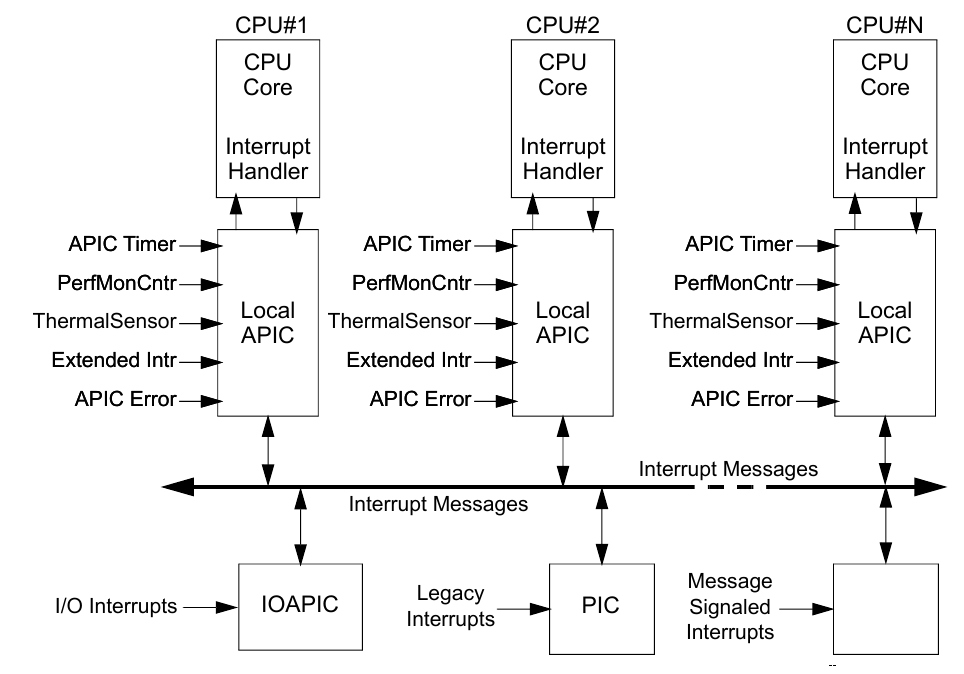
\includegraphics[width=.6\textwidth]{images/lapic_placeholder.png}
        \caption{Illustration of how \acrshort{a_lapic}s integrate in a multiprocessor system}
        \label{fig:state:technical:lapic}
    \end{center}
\end{figure}
\todo{This is a placeholder}

Intel later introduced the advanced programmable interrupt controller, short
APIC with its 486 processor line to allow the system to operate with multiple
CPUs. In modern CPUs, multiprocessor configurations are prevalent, and each processor
core has its own APIC. Because the APIC is CPU local, these APICs are called
local APICs or \gls{lapic}, short \acrshort{a_lapic}. \acrshort{a_lapic}s forward
interrupts from different sources to the respective CPU core. For example, the
\gls{lapic} receives interrupts such as \gls{ipi} (\acrshort{a_ipi}) from other
\acrshort{a_lapic}s, interrupts from devices connected to the IOAPIC, and legacy
interrupts from the PIC. Figure~\ref{fig:state:technical:lapic} shows a
schematic view on how the LAPIC of each CPU core integrates into the system.
System software must change the CPU to \gls{pmode} to
activate the \acrshort{lapic} system. After changing to \gls{pmode}, system
software must write a valid address to the APIC base address register. All APIC
registers are then mapped to the 4-KiB APIC register space starting at the
address specified in APIC base address register. System software can then access
APIC registers with memory reads and writes to the APIC register space.

